\documentclass{article}
\usepackage{graphicx}
\usepackage{geometry}
\usepackage{amsmath,mathpazo}
\usepackage{amssymb}
\usepackage{mathtools}
\usepackage{commath}
\usepackage{enumitem}
\usepackage{listings}
\usepackage{grffile}
\usepackage{hyperref}

\geometry{
  top=20mm,
}
\newcommand{\boldvec}[1]{\boldsymbol{\vec{\textbf{#1}}}}
\newcommand{\capvec}[1]{\boldsymbol{\hat{\textbf{#1}}}}
\newcommand{\bld}[1]{\textbf{#1}}
\newcommand{\ital}[1]{\textit{#1}}
\newcommand{\italb}[1]{\textbf{\textit{#1}}}
\begin{document}

\title{Machine Learning- COL774 \\Assignment 2}
\author{Ankesh Gupta\\2015CS10435}

\date{}
\maketitle

\section*{Naive Bayes Classifier}

% \bld{What was done:}
% \begin{enumerate}
% \item Batch Gradient Descent was implemented to train the given dataset.
% \item Different \ital{learning rates} and \ital{convergence values} were engineered.
% \item Loss functions were plotted and visualized.
% \end{enumerate}  
\bld{Observations:}
\begin{enumerate}
\item The test accuracy obtained on random prediction=$12.50\%.$ This is emperical averaged over 10 runs. This could well be guessed, as randomly, hitting a correct class during prediction has $probability=\frac{1}{8}$.
\item The test accuracy obtained on majority prediction=$20.08\%.$
\item The test accuracy obtained by our Naive Bayes classifier=$38.4\%$.
\item Our algorithm causes an $\approx26\%$ increase over random baseline and $\approx18.5\%$ increase over majority baseline.
\item Label 1 has highest value of diagonal entry. This means that this maximum correct predictions were made corresponding to this category.
\item Another category, that shines similar to Label 1 is Label 10, with $2^{nd}$ highest correct predictions.
\item  Studying the matrix, we realise that predictions for classes \{2,3,4\} got heavily biased towards class 1. Similar is the situation with classes \{7,8,9\} which tilted towards 10.
\item The reason for this bias could be the \italb{initial class imbalance} that our training data suffers from. 
\item Again, the accuracy obtained was $38.4\%$. No significant gains were observed. This might be because initial data cleaning might have removed very much the noise in the data. The class imbalance still remains. 
\item The bottleneck that algorithm is facing is loss of context so a negated good word is getting interpreted as good word and that is the root of the problem.
\item One of the feature engineering was to use combination of \italb{unigrams and bigrams} along with data augmentation and thresholding. Duplicates of data were added to training data to reduce class imbalance.
\item Accuracy obtained using this method was $38.9\%$.
\item Another method tried was \href{https://towardsdatascience.com/document-feature-extraction-and-classification-53f0e813d2d3}{\italb{TF-IDF}} in which experiments were repeated with and counts of words were replaced by their weights. The model again landed up showing accuracy $37\%$ accuracy when no augmentation was made, and $38\%$ accuracy with single augmentation.

\begin{figure}[h]
\vspace*{-2cm}
\centering
\includegraphics{ConfusionMatrix1.png}
\caption{Confusion Matrix without Stemming}
\end{figure}
\begin{figure}[h]
\vspace*{-2cm}
\centering
\includegraphics{ConfusionMatrix.png}
\caption{Confusion Matrix with Stemming and Stopwords removed}
\end{figure}
\clearpage
\item \italb{Bigram Model} turns out better because it in a sense includes partial context of word. One may argur that this logic would be better for $n-grams$ for $n>2$ but out input space grows exponentially, and hence the features become extremely sparse. If we had large data, probably $n-grams$ would out-perform.
\end{enumerate}

\section*{Support Vector Machine(SVM)}
\bld{Observations:}
\begin{enumerate}
	\item Test Accuracy obtained was $=92.54\%.$ Train Accuracy was $=94.1\%$.
	\item Accuracy in case of Linear Kernel $=92.78\%.$ Accuracy with Gaussian Kernel $=97.23\%.$
	\item Our implementation SVM compare fairly well with the inbuilt version. Their implementation attains a meagre $0.24\%$ improvement compared with our's. That could be taken care if we change the number of iterations for a classifier's convergence. Current limit$=2000$ iterations.
	\item Best value of $C=10$. Actually $C=5$ and $C=10$ both gives exact same results, but $C=10$ ran a bit faster.
	\item This value of $C$ also outperforms on the test set. Here is a tabulated form of above findings.
\begin{center}
 \begin{tabular}{||c|c|c||} 
 \hline
 C & Validation(\%) & Test(\%) \\ [0.5ex] 
 \hline\hline
 $10^{-5}$ & 71.59 & 72.11\\ 
 \hline
 0.001 & 71.59 & 72.11\\
 \hline
 1 & 97.355 & 97.23\\
 \hline
 5 & 97.455 & 97.29\\
 \hline
 10 & 97.455 & 97.29\\ [1ex] 
 \hline
\end{tabular}
\end{center}
	\item On a subtle note, analyzing the above scenario we realize that increasing $C$ is causing our classifier to classify more accurately.
	\item When $C$ is low, it indicates classifier that you are allowed to \italb{misclassify}, but the ones you classify correct much have large margin.
	\item As we increase $C$, it indicates to the classifier that our focus is now to \ital{classify more and more points accurately}, rather than separating the classes well.
	\item Class 9 faces most difficulty in classification as it has most number of misclassifications. 
	\item On visualizing, we see noisy 9 is quite similar to 4 and 7 at times, and it is natural for our model to breakdown to such granularity.
	\item Besides, 2 and 7 are the pair which confuses each other a lot.
	\item Visualization also shows how 2 and 7 our inter twined in some scenario and it becomes difficult even for human vision to distinguish unambiguously.
\end{enumerate}
\begin{figure}[h]
\vspace*{-2cm}
\centering
\includegraphics{Accuracy.png}
\caption{Accuracy for CrossValidation and Test}
\end{figure}
\begin{figure}[h]
% \vspace*{-1cm}
\centering
\includegraphics{mnist.png}
% \caption{Confusion Matrix with Stemming and Stopwords removed}
\end{figure}

\begin{figure}[h]
\vspace*{-2cm}
\centering
\includegraphics{2_7_1.png}
\caption{Correct-2 Pred-7}
\end{figure}
\begin{figure}[h]
\vspace*{-2cm}
\centering
\includegraphics{2_7_2.png}
\caption{Correct-2 Pred-7}
\end{figure}
\begin{figure}[h]
\vspace*{-2cm}
\centering
\includegraphics{2_7_3.png}
\caption{Correct-2 Pred-7}
\end{figure}
\begin{figure}[h]
\vspace*{-2cm}
\centering
\includegraphics{9_4_1.png}
\caption{Correct-9 Pred-4}
\end{figure}
\begin{figure}[h]
\vspace*{-2cm}
\centering
\includegraphics{9_4_2.png}
\caption{Correct-9 Pred-4}
\end{figure}
\begin{figure}[h]
\vspace*{-2cm}
\centering
\includegraphics{9_7_3.png}
\caption{Correct-9 Pred-7}
\end{figure}
\begin{figure}[h]
\vspace*{-2cm}
\centering
\includegraphics{7_2_1.png}
\caption{Correct-7 Pred-2}
\end{figure}

\begin{figure}[h]
\vspace*{-2cm}
\centering
\includegraphics{7_2_2.png}
\caption{Correct-7 Pred-2}
\end{figure}

% \item While observing the contours for different learning rates, it was observed that for lower learning rate, the jump between successive $epochs$ was comparatively lower that jump for rates.
% \item Direct consequence of above phenomenon was increased \ital{convergence time} as well as number of iterations for lower rates. However, increasing $\eta$ again raised the epochs because of oscillations.
% \item Another interesting observation was that for low learning rates, algorithm $stably$ converged to the minima, whereas for $\eta=0.017$, it first $oscillated$ about the minima a bit and then converged.
% \item It failed convergence for next $\eta=0.021$ as oscillations only pushed it further away from the minima.
% \item Epochs also increased with decrease in error condition($\epsilon$) kept for convergence.
% \item Optimal value of learning rate was around $\eta=0.09$ for below mentioned $\epsilon$.

% Here is a tabulated form for $\eta$ vs $epochs$ on the dataset, with $\epsilon=10^{-7}$, that is difference of $J(\theta)$ became less than $\epsilon$\italb{(Stopping Criteria)}. Obtained $\theta$ were: $$\theta_0 =0.9965$$ $$\theta_1 =0.0013$$



% \begin{figure}
% \vspace*{-2cm}
% \centering
% 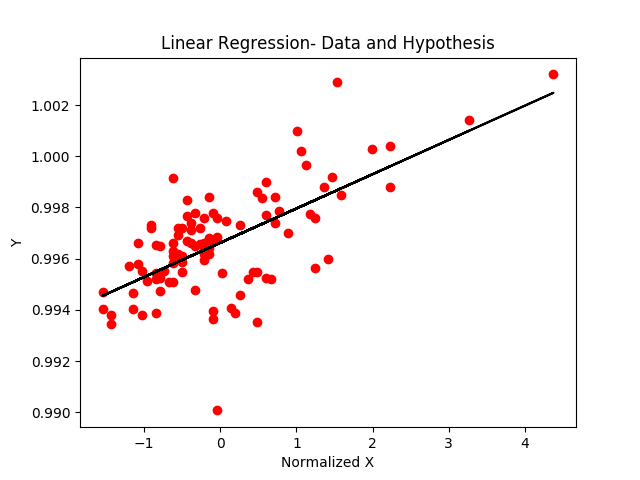
\includegraphics{Hypothesis.png}
% \caption{Example Plot of Hypothesis and data for $\eta=0.009$}
% \end{figure}

% \begin{figure}
% \vspace*{-2cm}
% \centering
% 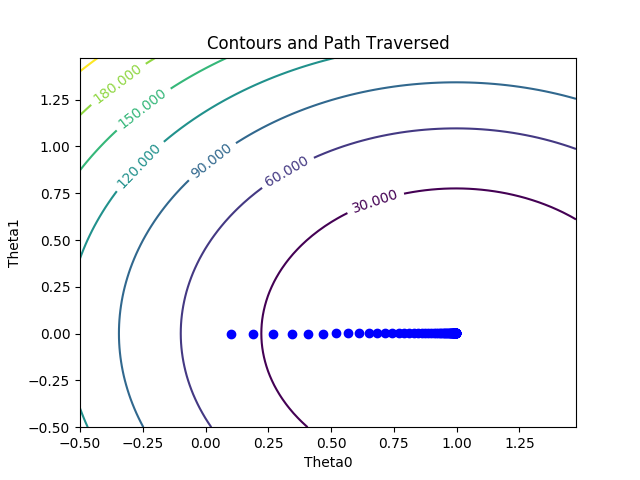
\includegraphics{Contours1.png}
% \caption{Example Plot of Hypothesis and data for $\eta=0.001$}
% \end{figure}

% \newpage


% \section*{Question 2}
% \bld{What was done:}
% \begin{enumerate}
% \item Closed form equations were implemented for linear regression and locally weighted linear regression$(LWLR)$.\italb{Bandwidth parameter} for LWLR($\tau$) was engineered.
% \item Inferences were drawn on extreme values of $\tau$.
% \end{enumerate}  

% \bld{Observations:}
% \begin{enumerate}
% 	\item The best value of $\tau$ was 0.3.
% 	\item Too low $\tau(<0.2)$ gave rise to $overfitting$. Too high $\tau(>5)$ resulted in $underfitting$. Example figure is shown.
% 	\item High $\tau$ makes the value in power of exponent $\approx 0$ which resulted in equal weightage of all sample points, a reduction of its power to \italb{Linear Regression}.
% 	\item Low $\tau$ assigns too much weight to the point in consideration and hence forces the hypothesis to fit as many points as it could, resulting in underfitting.
% 	\item Although powerful, this technique is \italb{computationally expensive}, as evaluation at each point is quite expensive. In our case, it required complete data lookup as well as $inverse$ computations.
% 	\item Closed form $\theta$ for Linear Case: \textbf{$\theta_0=0.9966$, $\theta_1=0.0013$}
% 	\item Closed form expression for LWLR is $$\theta=(W^TWX)^{-1}(X^TW^TY)$$
% \end{enumerate}

% \begin{figure}
% \vspace*{-2cm}
% \centering
% 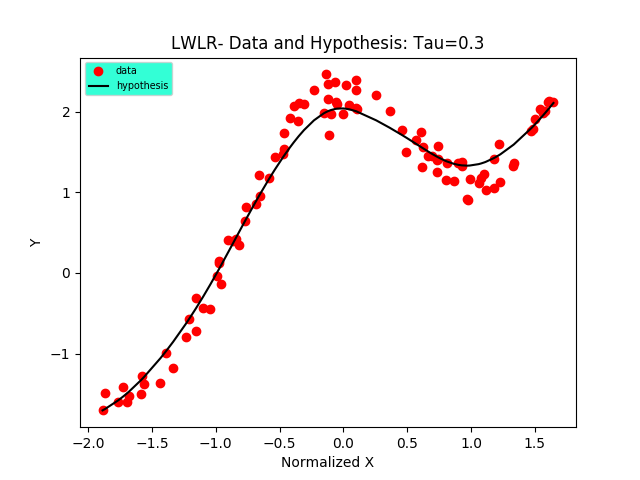
\includegraphics[scale=0.9]{LWLR_good.png}
% \caption{Best Fit}
% 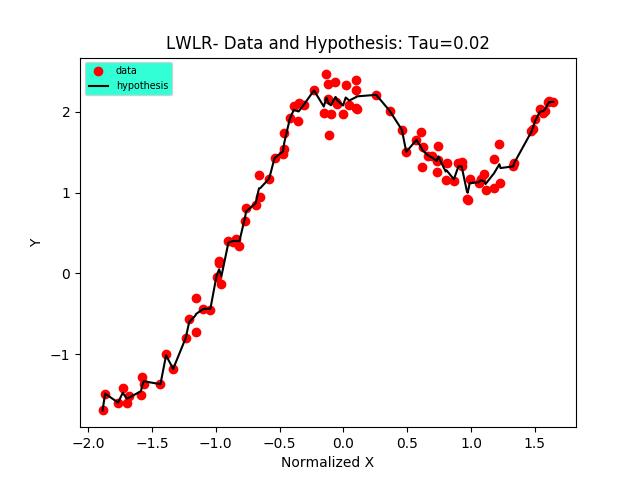
\includegraphics[scale=0.9]{LWLR_over.png}
% \caption{An example of small $\tau$}
% \end{figure}


% \begin{figure}
% \vspace*{-2cm}
% \centering
% 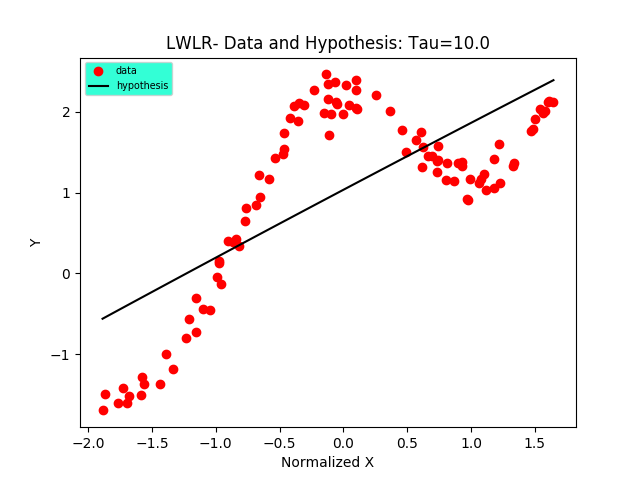
\includegraphics[scale=0.9]{LWLR_under.png}
% \caption{An example of large $\tau$}
% 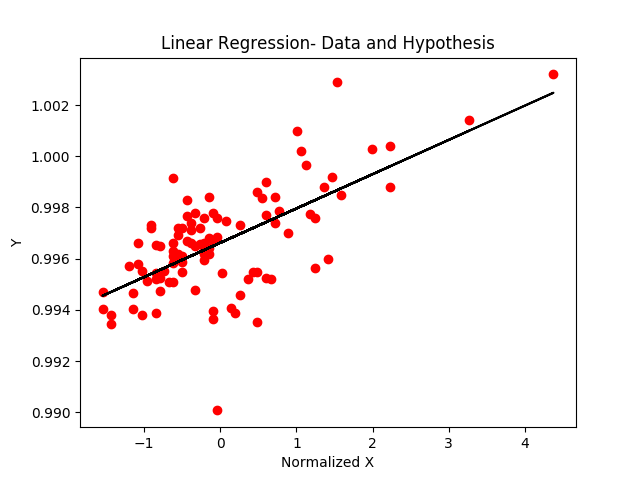
\includegraphics[scale=0.9]{AnalyticHypothesis.png}
% \caption{Hypothesis plot for Closed form of Linear Regression}
% \end{figure}


% % \newpage
% \section*{Question 3}
% \bld{What was done:}
% \begin{enumerate}
% \item Newton's method was applied to optimize/maximise $likelihood$ for the problem.
% \item Decision boundary was plotted and analyzed.
% \end{enumerate}  

% \bld{Observations:}
% \begin{enumerate}
% 	\item Obtained $\theta$ leading to covergence: $$\theta_0=0.401$$ $$\theta_1=2.588$$ $$\theta_2=-2.725$$
% 	\item The stopping criteria was when $\|\theta^t-\theta^{t-1}\|_2<\epsilon$
% 	\item Generally, Newton takes lower epochs than $Gradient Descent$ but computationally suffers because of computation of inverse of $Hessian$.
% 	\item A benefit of using it is we don't have to engineer any $step\_size$ or learning rate, as in \ital{Gradient Descent}.
% \end{enumerate}
% General tabulation of experiments done with different converging criteria($\epsilon$)
% \begin{center}
%  \begin{tabular}{||c|c||} 
%  \hline
%  $\epsilon$ & Epochs \\ [0.5ex] 
%  \hline\hline
%  0.1 & 8  \\ 
%  \hline
%  0.001 & 258 \\
%  \hline
%  $10^{-6}$ & 968 \\
%  \hline
%  $10^{-9}$ & 1687 \\
%  \hline
% \end{tabular}
% \end{center}

% \begin{figure}[h]
% \vspace*{-0.5cm}
% \centering
% 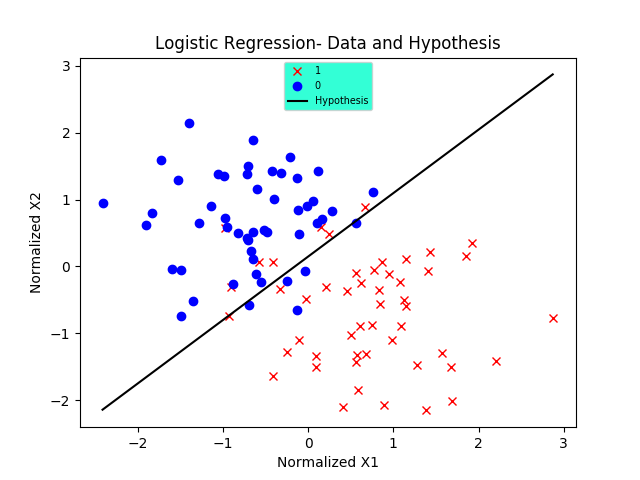
\includegraphics[scale=0.75]{Logistic.png}
% \caption{Decision Boundary and Points $\epsilon=10^{-6}$}
% \end{figure}

% \section*{Question 4}
% \bld{What was done:}
% \begin{enumerate}
% \item Closed form equations were derived for $\mu_0,\mu_1,\Sigma's,\phi$.
% \item Decision boundary equations were derived and plotted once assuming $\Sigma_0=\Sigma_1$, and other time, removing the restriction.
% \item The obtained boundaries were analyzed.
% \item Alaska is numbered $1$ and Canada, $0$.
% \end{enumerate}  

% Obtained values of $\mu's,\Sigma's,\phi$ on $normalized$ data are:
% \begin{align*}
% \phi &=0.5\\
% \mu_0&=\begin{bmatrix}
% -0.7553 & 0.685
% \end{bmatrix}\\
% \mu_1&=\begin{bmatrix}
% 0.7553 & -0.685
% \end{bmatrix}\\
% \Sigma&=\begin{bmatrix}
% 2.333 & 0.0988\\
% 0.0988 & 1.8886
% \end{bmatrix}\\
% \Sigma_0&=\begin{bmatrix}
% 0.4774 & 0.1099\\
% 0.1099 & 0.4135
% \end{bmatrix}\\
% \Sigma_1&=\begin{bmatrix}
% 0.3816 & -0.1548\\
% -0.1548 & 0.6477
% \end{bmatrix}\\
% \end{align*}

% Obtained Decision Boundary when $\Sigma_0=\Sigma_1$ is linear given by:

% \begin{align*}
% (\mu_1^T\Sigma^{-1}-\mu_0^T\Sigma^{-1})x&=0.5*(\mu_1^T\Sigma^{-1}\mu_1-\mu_0^T\Sigma^{-1}\mu_0) + \log{\frac{1-\phi}{\phi}}
% \end{align*}

% Obtained Decision Boundary without the above assumption is quadratic in nature given by:

% \begin{align*}
% x^T(\Sigma_1^{-1}-\Sigma_0^{-1})x+2(\mu_0^T\Sigma_0^{-1}-\mu_1^T\Sigma_1^{-1})x&=(\mu_0^T\Sigma_0^{-1}\mu_0-\mu_1^T\Sigma_1^{-1}\mu_1)+2*\log{\frac{\phi}{1-\phi}}-\log{\frac{|\Sigma_1|}{|\Sigma_0|}}
% \end{align*}

% \begin{figure}[h]
% \vspace*{-2cm}
% \centering
% 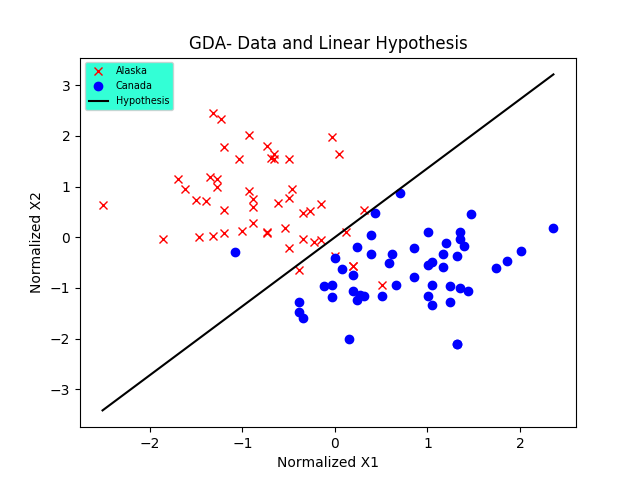
\includegraphics[scale=0.9]{GDALinear.png}
% \caption{Linear Fit when $\Sigma_0=\Sigma_1$}
% 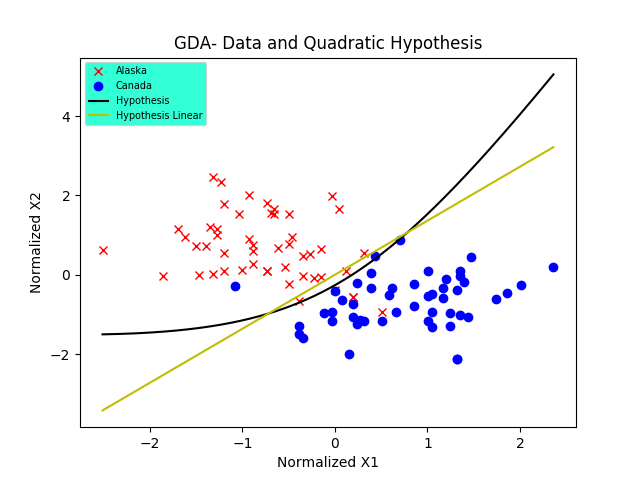
\includegraphics[scale=0.9]{GDAQuad.png}
% \caption{General GDA Quadratic Fit}
% \end{figure}

% Analyzing the decision boundary to comment which of them better fits is non-trivial given so few instances. But given so few a datapoints, if indeed the underlying $x/y \sim N(\mu,\sigma^2)$, then GDA is one of the better discriminator's because of its strong modelling assumptions. Both the \italb{boundaries} do a decent role in separating the given set of instances. Since the points are concentrated in a local neighbourhood for both the classes, their is a stray possibility that the underlying distribution is indeed $Gaussian$.

% Since the quadratic curve allows \italb{larger class of functions} to be estimated, we can say that quadratic boundary is a better estimator as it misclassifies very few data points. Also its quadratic curve is in a sense, better/strongly separating the 2 classes. But again, we definitely need more instances to comment something stronger.
% \begin{figure}[h]
% \caption{Example Plot of Contour for $\eta=0.019$}
% \centering
% 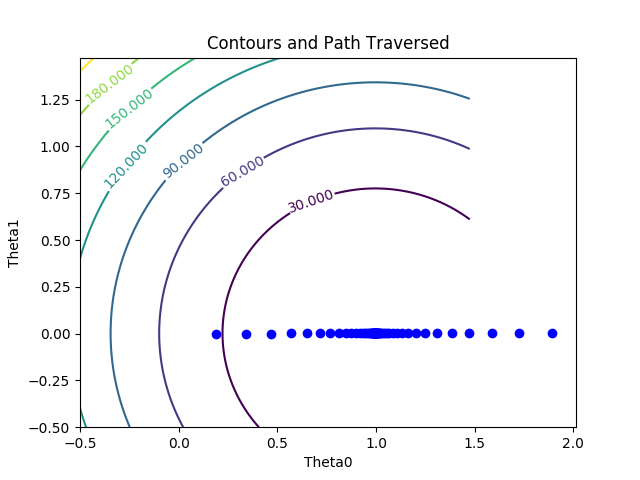
\includegraphics{Contours:Learning Rate=0.019.png}
% \end{figure}

% In an unpipelined setting, things are simpler. Each for-loop manipulation of z goes completely through the processor. The clock is unpipelined setting is 1 common clock, with 1 clock cycle period=$(2+1+1+1+1+1+2)ns=9 ns$. The loop executes 1000 times and thus, 
% \begin{align*}
% \Aboxed{T_{unpipelined} &=(1000*9)ns=9000ns}
% \end{align*}

% \bld{Extra Assumptions:}
% \begin{enumerate}
%   \item There are 7 stages in pipeline. They are in order as mentioned in question.
%   \item All stages of pipeline share the same clock. The clock period is dictated by the slowest step, which is $2ns$.
%   \item Above assumption also ensures no stalls in our execution pipeline.
%   \item 2-way Pipelined Processor is interpreted as 2 execution pipelines available parallely.
% \end{enumerate}

% In pipelined setting, $clock cycle=2ns$, but each instruction travels 7 stages, making in a way, $14ns$ per instruction. But because pipeline architechture exploits \bld{\ital{idealism of stages}}, in an amortized setting, we can obtain 1 instruction per cycle. Since each of the $z[i]$ computations are \bld{\ital{independent}} of each other, we can feed 2 instruction for adjacent computations in 2 pipelines available. Hence, in essence, each pipeline executes $500$ such instructions. One of them, for odd i's and the other, for even i's.
% \begin{align*}
% T_{pipelined} &=(6*2)ns(filling\_pipeline) + (500*2)ns\\
% \Aboxed{T_{pipelined} &=(1012)ns}
% \end{align*}

% \bld{Note:} The assumption of no bubble in extra assumption section may be relaxed. If clock cycle is reduced to$=1ns$, we realise that each fetch and store operation will lead to pipeline stalls. In such a scenario, pipeline filling takes$=7ns$ and after, each instruction execution is completed in $2ns$. Hence, total time in this case:
% \begin{align*}
% T_{modified\_pipelined} &=(5*1+2)ns(filling\_pipeline) + (500*2)ns\\
% \Aboxed{T_{modified\_pipelined} &=(1007)ns}
% \end{align*}

% The pipeline stages are shown for first calculations, which had no stalls.

% \hspace*{-2.4cm}
% \includegraphics[scale=0.55]{Pipeline.jpg}


% \section*{Question 2}
% \bld{Assumptions:}
% \begin{enumerate}
%   \item Since not clear from question, it is assumed that array is $integer array(size 1 word)$ of size $4000 X 4000$.
%   \item Prefetching's are ignored to keep calculations simpler.
%   \item Data fetched from DRAM is first loaded in cache, and then fetched from cache in subsequent cycles.
%   \item Pipeline type fetching from DRAM is ignored.
%   \item Again, for loop timings are ignored considering separate hardware taking negligible time.
% \end{enumerate}

% The problem will be simpler to deal with if we analyze each of the array's independently.\\\\
% For $z$ array, a memory access need to be made $once$ every $4$ times loop j executes. Rest 3 times, cache comes in handy.\\
% For $x$ array, a memory access need to be made $once$ every $4$ times loop k executes. Rest 3 times fetch is made from cache.\\
% For $y$ array, a memory access need to be made $once$ for every iteration of loop k. Since the access's are column major wise, no cache locality could be exploited.\\

% Clearly, if we look at k array, then in every 4 iterations of the loop, memory access is made $(4+1)=5$ times for $y(4\_times)$ array and $x(once)$ array respectively. Cache access is done $(4+4+4)=12$ times, 4 times for x,y and z respectively. Hence, for doing $4*2=8$ floating point operations(FLOP), $512 ns$ are required. Hence, in essence, we perform:

% \begin{align*}
% Performance &=(\frac{8}{512})GFLOPS\\
%             &=(0.0156)GFLOPS\\
%             &=(15.6)MFLOPS
% \end{align*}

% \bld{Note:} z DRAM access are kept out of calculation as DRAM access are made once in every ((4*SIZE)*2) floating point operations, to which it has negligible contribution

% \section*{Question 3}
% Option \bld{2} is correct. The following sequence of events will lead to a \bld{deadlock} situation between the threads. Execute and Loops at below are used with respect to Statement No. mentioned in the question.

% \begin{enumerate}

%   \item Thread 1 executes 1,2,3,4,5. Loops at 5. $process\_arrived=1$
%   \item Thread 2 executes 1,2,3,4,5. Loops at 5. $process\_arrived=2$
%   \item Thread 3 executes 1,2,3,4,5 ($process\_arrived=3$,breaks),6,7,8,12,1 \ital{(successive invocation)},2,3,4,5. Loops at 5. $process\_arrived=4, process\_left=1$
%   \item No other thread ever breaks free of the loop as $processed\_arrived$ will never be reset again
% \end{enumerate}
  
% The sequence of operations above leads to \bld{deadlock}, where no thread is able to make any progress. This situation arise because 2 barrier in invocations are used in immediate succession(noted in point 3)\\

% The following code is one of the ways of resolving the issue pointed out above.

% \begin{verbatim}
% void barrier ( void ) {
%   L( S ) ;
%   process_arrived++;
%   UL( S ) ;
%   while ( process_arrived!=3) ;
%   L( S ) ;
%   process_left++;
%   UL( S ) ;
%   if(process_left==3){
%     process_arrived=0;
%     process_left=0;
%   }
%   while(process_left!=0);
% }
% \end{verbatim}

% The above code ensures that all the 3 threads executing the barrier leaves the barrier simultaneously. The flaw in previous snippet was that it synchronised threads momentuously, but their exiting the barrier was independent. Now, the barrier will ensure that all variables have been reset, and even the last thread in opertion pipeline is ready to depart.

% % \pagebreak

% \section*{Question 4}

% Option \bld(b) is correct.\\

% \begin{minipage}{0.5\textwidth}
%  \begin{lstlisting}
%   ****Thread i****
% while (true) {
% 1. flag[i]=true;
% 2. turn=j;
% 3. while(flag[j]==true && turn==j);
%    /∗ enter critical section
%    perform actions
%    exit */
% 4. flag[i]=false ;
%    } 
% \end{lstlisting}
% \end{minipage}
% \begin{minipage}{0.5\textwidth}
%  \begin{lstlisting}
%   ****Thread j****
% while (true) {
% flag[j]=true;
% turn=i;
% while(flag[i]==true && turn==i);
% /∗ enter critical section
% perform actions
% exit */
% flag[j]=false ;
% } 
% \end{lstlisting}\end{minipage}


% \bld{Justification of Exclusion:} Suppost for sake of contradiction, we assume that both the threads execute critical section simultaneously. WLOG, we assume that thread i executed statement 2 first. So, for thread j to execute critical section, flag[i] must have been false in while loop \bld{(..a)}. If we construct a \bld{happen-before} graph, we realise that Thread i statement 2 must happen before Thread j statement 2(assumption), which must happen before Thread j statement 3(sequentiality), which must happen before Thread i statement 1\bld{(from (..a))}. 

% Hence there is a \ital{happen-before loop, which leads to contradiction}. Notice here we assumed the an order of execution of Statement 2 WLOG, hence this completes the proof.\\

% \bld{Justification of Liveliness:} Its clear that if only 1 thread is invoking the function, the other threads flag remains false, and thread works uninterrupted. Interesting is when both threads want to access the critical section. Again, the while loop construct ensures that none of the threads executes the critical section in succession, keeping the other thread waiting. Each resetting of \ital{turn} variable is an opportunity for the waiting thread to complete its request of critical section.



% \section*{Question 5}
% \begin{enumerate}[label=(\alph*)]

% \item Lets start by writing the efficiency equation for given system, and doing algebraic manipulations.

% \begin{align*}
% E &=\frac{T_{serial}}{p*T_{parallel}}
% \end{align*}
% Substituting from the question, $T_{parallel}$, we get:
% \begin{align*}
% E &=\frac{T_{serial}}{T_{serial}+p*T_{overhead}}\\
%   &=\frac{1}{1+\frac{p*T_{overhead}}{T_{serial}}}
% \end{align*}
% We know that $T_{serial}$ is same as $W$(input size), the workload, which gives us:
% \begin{align*}
% E &=\frac{1}{1+\frac{p*T_{overhead}}{W}}
% \end{align*}
% Assuming that $T_{overhead}$ is a \bld{sublinear} function of Workload$(W)$, the growth in workload dominates the growth in overhead, which decreases the denominator, in turn increasing efficiency. Asymtotically we can write:
% \begin{align*}
% E &=\frac{1}{1+\frac{p*T_{overhead}}{W}} \approx{1}
% \end{align*}

% Hence, as input size grows, $Efficiency$ increases, and aymtotically reaches 1. The main assumption is that: $$W = \Omega({T_{overhead}})$$

% \item \bld{Scalability} is defined as the ability of parallel system to keep efficiency, when processing units and workload of the system changes.

% Lets analyze the given parallel construct and derive iso-efficiency function.

% \begin{align*}
% E &=\frac{T_{serial}}{p*T_{parallel}}\\
%   &=\frac{n}{n+p*\log_2 p}
% \end{align*}
% Moving terms, and writing $n$ as function of $p(processing units)$, we get:  
% \begin{align*}
% n &=\frac{E}{1-E}*p\log_2 p\\
% \end{align*}
% Let initial processing units be $p_1$, and later it changed to $p_2=k*p_1$, corresponding $n_1,n_2$ are:
% \begin{align*}
% n_1 &=\frac{E}{1-E}*p_1\log_2 p_1\\
% n_2 &=\frac{E}{1-E}*k*p_1\log_2 (k*p_1)\\
% \Aboxed{\frac{n_2}{n_1} &= k*(1+\frac{log_2 k}{log_2 p_1})}
% \end{align*}

% Although the system is scalable(because it are able to maintain \ital{isoefficiency}), it is \bld{weakly scalable}. This is because increase in $workload($n$)$ required to attain iso-efficiency is $super-linear$ with respect to processing units, as visible from the last equation. Hence the system is \bld{\ital{weakly scalable}}.

% \item The cost optimal version of parallel-sum algorithm for $n$ numbers on $p$ processing units does the following:

% \begin{enumerate}[label=(\roman*)]
% \item Divide the numbers $equally$ and $exclusively$ amongst the p cores. Each core get $\frac{n}{p}$ numbers.
% \item Sum all the numbers each core receives and store the sum locally. This takes $O(\frac{n}{p})$ time.
% \item Merge the local sums from each of the cores into a global sum in \ital{divide and conquer} style. This takes $O(log_2 p)$ time.
% \end{enumerate}  

% Examining the above algorithm, running time of above algorithm is $T_{parallel}=O(\frac{n}{p} + \log_2 p)$. The best serial algorithm sums up the numbers in $T_{serial}=O(n)$ time. Analyzing the cost: 
% \begin{align*}
% C_{s} &=T_{serial}=n\\
% C_{p} &=p*T_{parallel}=n+p*\log_2 p\\
% \frac{C_{p}}{C_{s}} &=1+\frac{p*\log_2 p}{n}
% \end{align*}

% As long as $n=\Omega(p*\log_2 p)$, the above parallel construct is cost optimal, as then asymtotically:
% \begin{align*}
% \Aboxed{C_p &=\Theta(C_s)}
% \end{align*}
% \end{enumerate}

% Deriving expressions for terms asked in question, $T_{parallel}$ has already been written above in runtime analysis. Substituting the values for summing,

% \begin{align*}
% T_{parallel} &=\frac{n}{p} + \log_2 p\\
%   &= \frac{n}{p}*1 + \log_2 p*(20+1)(Substituting)\\
% \Aboxed{T_{parallel} &= \frac{n}{p} + \log_2 p*(21)}
% \end{align*}

% For \bld{speedup($S$)},
% \begin{align*}
% S &=\frac{T_{serial}}{T_{parallel}}\\
%   &= \frac{n}{\frac{n}{p}+log_2 p}\\
% \Aboxed{S &= \frac{p}{1+\frac{p*log_2 p*21}{n}}} (Substituting)
% \end{align*}
% For \bld{efficiency($E$)},
% \begin{align*}
% E &= \frac{T_{serial}}{p*T_{parallel}}\\
%   &= \frac{n}{p*(\frac{n}{p}+log_2 p)}\\
%   &= \frac{n}{n+p*\log_2 p}\\
%   &= \frac{n}{n+p*\log_2 p*21}(Substituting)\\
% \Aboxed{E &= \frac{1}{1+\frac{p*\log_2 p*21}{n}}}
% \end{align*}

% Equations for \bld{Cost} had been derived while prooving optimality. What remains is substitution of time.
% \begin{align*}
% C_{s} &=T_{serial}=n\\
% C_{p} &=p*T_{parallel}=n+p*\log_2 p*21\\
% \Aboxed{\frac{C_{p}}{C_{s}} &=1+\frac{p*\log_2 p*21}{n}}
% \end{align*}

% \bld{Iso-efficiency} can be derived from Efficiency equation, by algebraic manipulations.
% \begin{align*}
% E &= \frac{n}{p*(\frac{n}{p}+log_2 p*21)}\\
% n*(1-E) &= E*p*log_2 p*21\\
% \Aboxed{n &= \frac{E}{1-E}*p*log_2 p*21}\\
% \end{align*}

\end{document}
